\chapter{提案手法におけるその他の工夫}
\label{sec:switch}

提案手法における工夫点として,Last Tag Prediction(LTP)とレジスタ・フリー・リストのセグメント化という 2 つ手法に関して評価を行った.本章では,これらの手法に関して説明を行う.

\section{LTP:Last Tag Prediction}
CONSARVARTIVE 方式 において,第 1 ソース・タグと第 2 ソース・タグがどちらもレディでない命令は,以下のアルゴリズムでセグメントを選択すると述べた.

\begin{itemize}
  \item サブ・セグメントを使用しない場合:第 1 ソース・タグでセグメントを選択する.選択したセグメントに空きがない場合,スワップして第 2 ソース・タグをもとにセグメントを決定する.なおも空きがない場合はストールする.
  \item サブ・セグメントを使用する場合:第 1 ソース・タグでメイン・セグメントを,第 2 ソース・タグでサブ・セグメントを選択する.選択したセグメントに空きがない場合,スワップを行い,第 2 ソース・タグでメイン・セグメントを,第 1 ソース・タグでサブ・セグメントを選択する.スワップしてなおも空きがない場合はストールする.
\end{itemize}

このアルゴリズムにおいて,スワップする場合としない場合に選択されるセグメントのどちらにも空きがある場合を考える.このような場合,CONSERVATIVE のアルゴリズムでは,スワップを行わずにディスパッチするセグメントを決定する.

このような場合に,レディとなるのがより遅く,比較がより多く行われるソース・オペランドのタグ(ラスト・タグ)を第 1 ソース・タグのフィールドに書き込むようにセグメントを選択すれば,タグ比較回数をより多く削減できると考えられる.ただし,ラスト・タグがどちらになるかという情報はデコード時にはわからないため,予測を行う必要がある.

ラスト・タグの予測方法は,論文~\cite{ernst2002}で提案されている.この方法を Last Tag Prediction(LTP)と呼ぶ.以下,LTP による予測とセグメントの選択方法に関して説明する.

\begin{figure}[htb]
  \centering
  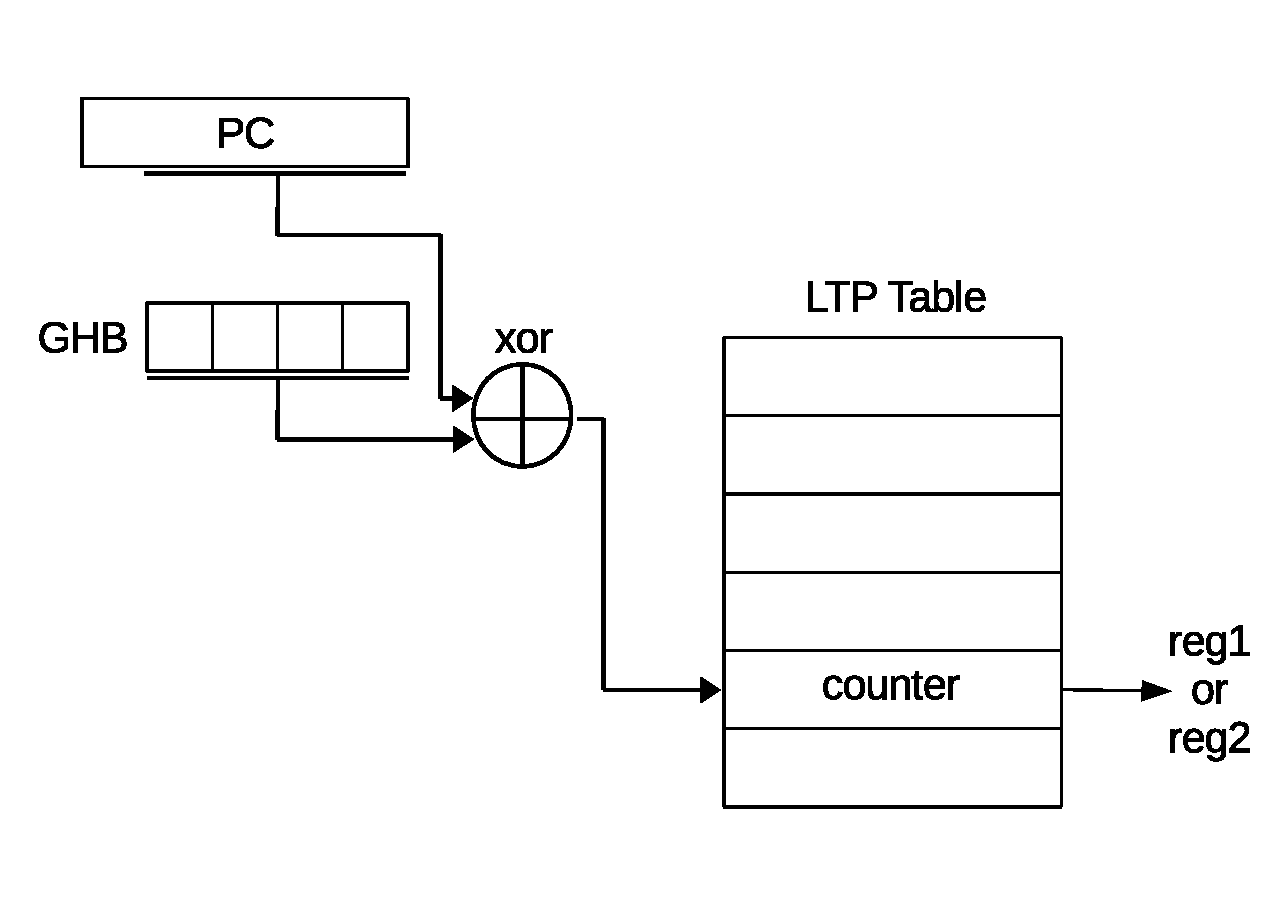
\includegraphics[keepaspectratio, scale=.8]{ltp}
  \caption{LTP の構成}
  \label{fig:ltp}
\end{figure}

LTP は,\fig{ltp}のように.命令の PC の下位ビットビットとグローバル分岐履歴(GHB:Global History Buffer)のハッシュをインデクスとするテーブル(LTP Table)で構成される.LTP Table の各エントリは 2 ビットの飽和型アップ・ダウン・カウンタで構成され,このカウンタは,値が 0 または 1 の場合に第 1 ソース・タグがラスト・タグであることを示し, 2 または 3 の場合に第 2 ソース・タグがラスト・タグであることを示す.予測と学習の方法について説明する.
  
\subsection{予測方法}
命令ディスパッチ時に,第 1 ソース・タグと第 2 ソース・タグがともにレディでなく,なおかつスワップした場合としない場合に選択されるセグメントがいずれもディスパッチ可能な場合に予測が行われる.予測の際には,PC と GHB のハッシュを用いてテーブルを検索し,該当するエントリのカウンタ値を読み出す.

第 1 ソース・タグがラスト・タグであると予測された場合には,スワップを行なわずにセグメントを選択しディスパッチする.第 2 ソース・タグがラスト・タグであると予測された場合には,スワップを行いセグメントを選択し,ディスパッチする.
  

\subsection{学習方法}
学習は命令発行時に,ディスパッチ時に予測を行った命令でのみ行われる.命令発行時に,第 1 ソース・タグと第 2 ソース・タグがレディとなったサイクルを比較する.第 1 ソース・タグ のほうが遅かった場合にはカウンタをデクリメントし,第 2 ソース・タグのほうが遅かった場合にはカウンタをインクリメントする.

\section{レジスタ・フリーリストのセグメント化}
提案手法による IQ の容量効率の低下を抑制するには,命令が各セグメントに均等に割り当てられるようにすればよいと考えられる.割り当てられるセグメントは,命令のソース・タグの値によって決定されるため,ソース・タグの下位ビットに偏りをなくすことができれば,命令は各セグメントに対して均等に割り当てられる.

ソース・タグの値はプログラムに依存するものであるため,ソース・タグの下位ビットを完全に均等にするということは難しいが,ディスティネーション・タグのリネームを工夫することによって,間接的にソース・タグの下位ビットの偏りをなくすことがで切ると考えられる.

これを実現する手法として,レジスタ・フリーリストのセグメント化を提案する.本手法では,レジスタのフリー・リストを IQ のセグメント数と同じ数だけセグメント化し,ディスティネーション・タグの下位ビットが均等になるようにリネームを行う.

本章では,まずレジスタ・フリーリストの基本事項に関して説明したのち,セグメント化したレジスタ・フリー・リストの動作とそのバリエーションに関して説明する.

\subsection{レジスタ・フリー・リスト}
レジスタ・フリー・リストは,現在使用されていない物理レジスタ番号を保持するスタック・バッファである.命令ノリネーム時に,フリー・リストから値を読み出し,その番号を命令のディスティネーション・オペランドのタグとする.命令乗リタイア時に ROB からタグが変換され,スタック・バッファに書き込まれる.

\begin{figure}[htb]
  \centering
  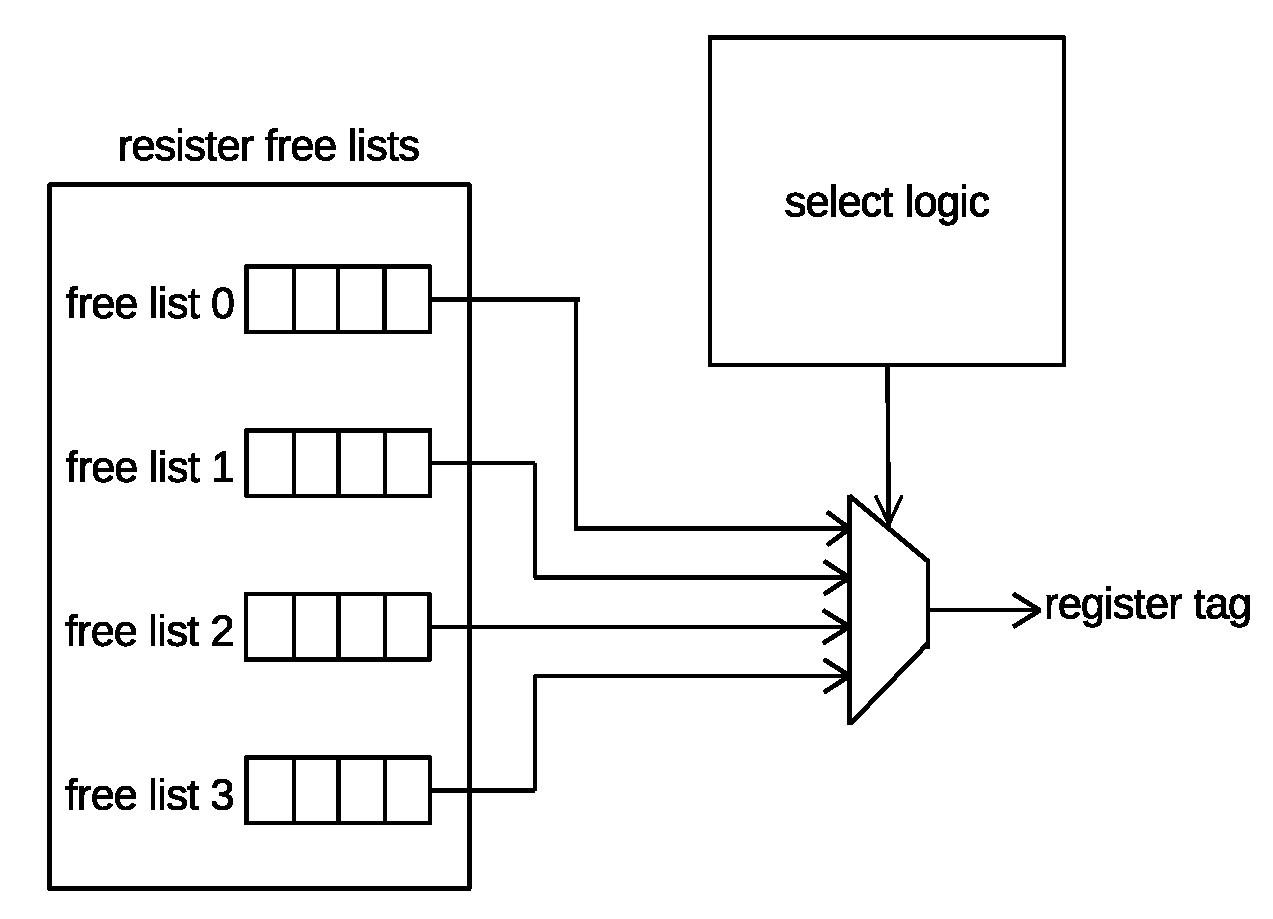
\includegraphics[keepaspectratio, scale=.8]{reg_flist}
  \caption{セグメント化したレジスタ・フリー・リスト}
  \label{fig:reg_flist}
\end{figure}

\subsection{セグメント化したレジスタ・フリー・リスト}
\fig{reg_flist}にセグメント化したレジスタ・フリー・リストを示す.本手法では,レジスタ・フリー・リストを,IQ のセグメント数と同数のセグメントに分割する.そして各セグメントには,タグの下位ビットがセグメントの番号と一致するタグを格納する.リネーム時には,読み出すセグメントを何らかのアルゴリズムより決定し,決定されたレジスタ・フリー・リストよりタグを読み出す.

タグを読み出すセグメントを均等に選択するアルゴリズムとしては,以下の 2 つが考えられる.
\begin{itemize}
  \item RANDOM:ランダムにセグメントを選択
  \item RAUNDROBIN:ラウンドロビンでセグメントを選択
\end{itemize}

また,より高度な選択の方法として,次のアルゴリズムが考えられる.
\begin{itemize}
  \item MAX:IQ のセグメントのうち,最も空きの多いセグメントと同じ番号のレジスタ・フリー・リストを選択
\end{itemize}


これは,タグを均等にする戦略とは異なる選択方法であるが,リネームされたレジスタがソース・オペランドとなる命令が,最も空きの多いセグメントにディスパッチされるようになるため,IQ がストールする確率を低下させることができ,有効であると考えられる.

\subsection{サブ・セグメントとの併用}
サブ・セグメントを使用する場合におけるレジスタ・フリー・リストのセグメント化に関して説明する.この場合,レジスタ・フリー・リストは IQ のメイン・セグメントの数と同数にセグメント化する.また,MAX のアルゴリズムにおいては,最も空きの多いメイン・セグメントと同じ番号のレジスタ・フリー・リストからタグを読み出す.